\documentclass[a4paper]{scrartcl}

\usepackage[T1]{fontenc}
\usepackage[utf8]{inputenc}
\usepackage[ukenglish,nswissgerman]{babel}
\usepackage[onehalfspacing]{setspace}
\usepackage{makeidx}
\usepackage{graphicx}

\setcounter{secnumdepth}{3}
\makeindex

\title{Sequenzen in \emph{Das Wohltemperierte Klavier, 1.~Band} von J. S. Bach}
\subtitle{Kontrapunktische Analysen von Modellen, Synkopendissonanzen und deren Verzierungen in ausgewählten Sequenzen aus den Fugen}
\subject{Musiktheoretischer Artikel}
\author{
	Wolfgang Drescher\thanks{Klasse: Dr. Felix Diergarten}\\
	Hochschule für Musik Freiburg
}
\date{\today}


\begin{document}

\maketitle

\tableofcontents

\section{Einleitung}

Im Musiktheorie Unterricht beschäftigen wir\footnote{Im gemeinsamen Musiktheorie-Unterricht von Adrian Nagel und mir, bei Prof. Dr. Felix Diergarten} uns in diesem Semester\footnote{Wintersemester 2017/2018} mit Fugen und versuchen neben dem eigenen nachkomponieren, angelehnt an Bachs Wohltemperiertes Clavier, auch mit wöchentlichen Analysen von Bachs Fugen aus dem ersten Band Satztechniken und Methoden zu finden, mit denen wir unsere eigenen Stilkopien an den Sound von Bach annähern können.
Im Zuge dessen sind uns immer wieder Stellen aufgefallen, die durch besondere Bezifferungen und Kontrapunktik einen sehr Bach typischen Klang erzeugen.
Die eindrücklichsten dieser Stellen sollen in diesem Artikel aufgezeigt und analysiert werden.


\subsection{Problemstellung}

Viele der von uns angesehenen Traktate geben ausführliche Informationen, wie eine Fugenexposition aufgebaut ist, besonders wie der der Comes eingerichtet werden muss, aber es liessen sich kaum Stellen finden, wie der weitere Verlauf einer Fuge aufgebaut ist.
Erwin Ratz schreibt in seiner Formenlehre\autocite[21]{ratz:formenlehre} von zwei grundlegenden Grundprinzipien in Instrumentalformen: \emph{fester Gefügtes} und \emph{locker Gefügtes}.
Er versucht zu zeigen, dass Beethoven nicht als Gegensatz zu Bach empfungen werden soll, sondern als organische Weiterentwicklung.
Während \emph{fester gefügten} Teile die z.B. dem Hauptsatz einer Sonate oder der Exposition einer Fuge relativ klar definierten Kompositionsprinzipien folgen, bleiben, nicht nur bei Ratz, die Teile dazwischen unscharf erklärt.
Es ist deshalb besonders schwer, bei eigenen Stilkopien die Sequenzen zwischen den Durchführungen, seien diese nur harmonische Sequenzen\footnote{Damit meine ich Stellen, die nur harmonisch den Stationen einer Sequenz wie etwas einem Quintfall folgen, aber Rhythmisch nicht so aufgebaut sind, dass diese als regelmässige Sequenzierungen wahrgenommen werden, da keine Teile wörtlich auf einer anderen Stufe transponiert erklingen.}, oder tatsächlich wörtlich sequenzierte Abschnitte, näher am Vorbild der Bach Fugen nach zu komponieren, ohne dass sich diese Sequenzen eher anhören die Sequenzen aus den Triosonaten von Arcangelo Corelli.


\subsection{Ziel dieses Artikels}

An diesem Punkt soll dieser Artikel ansetzten.
Um ein besseres Verständnis dafür zu bekommen, wie genau Bach solche formal nicht streng definierten Stellen komponiert und warum diese den für Bach so typischen Tonfall haben, werden in diesem Artikel ausgewählte Sequenzen kontrapunktisch analysiert und versucht auf die üblichen Sqeuenzes der Genegalbass Epoche zurückzuführen.
Ich hoffe dabei dem Leser Möglichkeiten mitzugeben, wie innerhalb einer Fuge die verschiedenen Durchführungen durch Sequenzen miteinander verbunden werden können und wie man diese durch Verzierungen, Variationen oder mit \emph{theatralischen Dissonanzauflösungen}\autocite[208-219]{heinichen:general-bass,menke:kontrapunkt2} in einen klanglichen Charakter bringen kann der näher an Bachs Stil ist als das blosse Sequenz-Modell mit seinen üblichen Verzierungen.


\subsection{Vorgehensweise}

Um dem angehenden Komponisten von Fugen im Stile Bachs Rezepte mit auf den Weg zu geben, wie solche Sequenzen selbst nachgebaut werden können, habe ich bei den Analysen stets versucht das zu Grunde liegende Sequenz-Modell auf dessen kontrapunktischen Kern zurückzuführen und dieses dann Stück für Stück wieder mit Verzierungen, \emph{transitus } und Varianten anzureichern bis am Ende wieder die originale Komposition von Bach herauskommt.

Ich versucht damit keineswegs den Gegankengang von Bach beim Komponieren zu reproduzieren.
Vielmehr soll so für den Stilkopisten ein Weg gezeigt werden, wie duch Änderungen in der Generalbass-Bezifferung oder im Kontrapunkt so eine Stelle entsprechend simuliert werden kann.

\section{Fuge in g-moll, BWV 861, T.~24ff}

Fast hätten wir bei unseren Analysen im Unterricht diese Fuge ausgelassen, da sie -- wahrscheinlich spätestens seit den Analysen von Erwin Ratz -- als Paradebeispiel für die Form von Bach Fugen verwendet wurde.

\begin{quote}
"<Dem Schema am nächsten steht die \emph{g-moll Fuge} des ersten Bandes.">\autocite[80f]{ratz:formenlehre}
\end{quote}

Wir wollten aber durch eigene Analysen herausfinden, warum diese Fuge als Lehrbeispiel so gut geeignet ist.
Unsere Untersuchungen haben ergeben, dass dies wahrscheinlich deshalb so ist, weil die Durchführungen sehr regelmässig aufgebaut sind und einem klaren Tonartenplan folgen\footnote{1.~Durchführung in \emph{g-moll}, 2.~Dfg. in \emph{B-dur}, 3.~Dfg. in \emph{c-moll}, 4. und 5.~Dfg. wieder in \emph{g-moll}}.
Ausserdem geht die 2.~Durchführung noch einmal, fast wie in der Exposition, durch alles Stimmen, abgesehen davon, der 4.~Themeneinsatz in T.~17 in der Tenorlage hier erneut als Basseinsatz erklingt.
Ein weiterer Punkt wäre, dass diese \emph{Fuga à 4 voci} erst recht spät in der 2.~Durchführung ab Takt 15 tatsächlich vierstimmig ist und vorher maximal drei Stimmen erklingen, was vorallem in der Exposition einer vierstimmigen Fuge etwas überrascht.

Eher untypisch ist bei dieser Fuge hingegen, dass zwischen den Durchführungen keine regelmässigen Sequenzen komponiert sind, sondern nur Orgelpunkte, Kadenz-Modelle und \emph{harmonische Sequenzen}.
Erst am Ende der Fuge zwischen den beiden letzten Durchführungen, beide in \emph{g-moll}, erklingt eine regelmässige Sequenz die mit drei Sequenzgliedern sogar relativ lang ist.
Durch die besondere ausarbeitung Bachs der Dissonanzen und Verzierungen in dieser Romanesca-Sequenz\index{Romanesca} sollen im folgenden genauer untersucht werden.
In Abbildung~\ref{fig:bwv681-original} das Notenbeispiel dazu.

\begin{figure}[htbp]
	\centering
	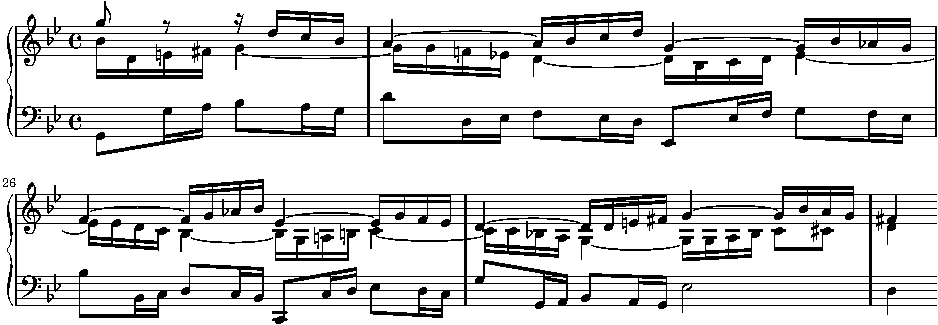
\includegraphics{lilypond/g-moll/render/original}
	\caption{Fuge in g-moll, BWV~861, T.~24ff}
	\label{fig:bwv681-original}
\end{figure}

Um einen Ausgangpunkt für weitere Analysen zu haben sei in Abbildung~\ref{fig:bwv681-romanesca-standard} die Standard Romanesca über Bachs Bass mit der üblichen 4--3 9--8 Bezifferung gegeben.

\begin{figure}[htbp]
	\centering
	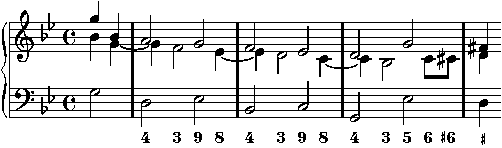
\includegraphics{lilypond/g-moll/render/romanesca-standard}
	\caption{Typische Romanesca mit 4-3-consecutive}
	\label{fig:bwv681-romanesca-standard}
\end{figure}

Lorem ipsum dolor sit amet, consectetur adipisicing elit, sed do eiusmod tempor incididunt ut labore et dolore magna aliqua. Ut enim ad minim veniam, quis nostrud exercitation ullamco laboris nisi ut aliquip ex ea commodo consequat. Duis aute irure dolor in reprehenderit in voluptate velit esse cillum dolore eu fugiat nulla pariatur. Excepteur sint occaecat cupidatat non proident, sunt in culpa qui officia deserunt mollit anim id est laborum.

\begin{figure}[htbp]
	\centering
	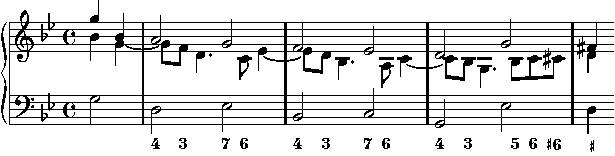
\includegraphics{lilypond/g-moll/render/romanesca-vorhalte}
	\caption{Bachs Harmonisierung der Romanesca-Sequenz in der Fuge in g-moll, BWV~861, T.~24ff}
	\label{fig:bwv681-vorhalte}
\end{figure}

Lorem ipsum dolor sit amet, consectetur adipisicing elit, sed do eiusmod tempor incididunt ut labore et dolore magna aliqua. Ut enim ad minim veniam, quis nostrud exercitation ullamco laboris nisi ut aliquip ex ea commodo consequat. Duis aute irure dolor in reprehenderit in voluptate velit esse cillum dolore eu fugiat nulla pariatur. Excepteur sint occaecat cupidatat non proident, sunt in culpa qui officia deserunt mollit anim id est laborum.


\printindex

\renewcommand{\indexname}{Stichwortverzeichnis}
\addcontentsline{toc}{section}{Stichwortverzeichnis}
\listoffigures

\end{document}
